\documentclass[a4paper]{article}
\usepackage[margin=1in]{geometry}
\usepackage[fontset=founder]{ctex}
\usepackage{anyfontsize}
\usepackage{graphicx}
\usepackage{amsmath}
\usepackage{mathabx}
\usepackage{multirow}

\graphicspath{{../figures/}}

\title{\textbf{霍尔效应}}
\author{姚苏航\quad PB22061220\\实验时间: 2023年11月6日}
\date{}

\begin{document}

    \maketitle

    \paragraph{摘要:}
    {
        霍尔效应指在磁场中的载流导体上出现横向电势差的现象。
        本实验对霍尔效应进行研究并利用霍尔效应进行各种分析和测量工作,
        测量了待测霍尔片的霍尔系数、横向电导率、载流子类型及浓度和载流子迁移率;
        使用对称测量法来消除副效应影响, 并绘制了锑化铟片的$V_H-I_M$曲线。
    }

    \paragraph{关键词:}
    {
        霍尔效应, 爱廷豪森效应, 锑化铟片
    }

    \vspace{1cm}


    \section{实验原理}\label{sec:3}

    \subsection{通过霍尔效应测量磁场}

    {
        霍尔效应装置如图1和图2所示。
        将一个半导体薄片放在垂直于它的磁场中(B的方向沿z轴方向),
        当沿$y$方向的电极$C$、$D$上施加电流$I$时,
        薄片内定向移动的载流子(设平均速率为$u$)受到洛伦兹力$F_B$的作用:
        \begin{equation}
            F_B=quB\label{eq:equation}
        \end{equation}
    }\label{subsec:7}

    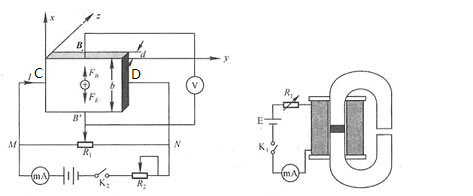
\includegraphics[height=0.255\textheight]{1_2}

    \hspace{2.6cm}{\small 图一}\hspace{6.8cm}{\small 图二}

    {
        无论载流子是负电荷还是正电荷,$F_B$的方向均沿着x方向,
        在磁力的作用下, 载流子发生偏移, 产生电荷积累,
        从而在薄片B、B'两侧产生一个电位差$V_H$, 形成电场$E$。
    电场使载流子受到一个与$F_b$方向相反的电场力$F_E$:
        \begin{equation}
            F_E=qE=q\frac{V_H}{b}\label{eq:equation4}
        \end{equation}
    }

    {
        其中b为薄片宽度, $F_E$随着电荷累积而增大,
        当达到稳定状态时$F_E=F_B$, 即
        \begin{equation}
            quB = q\frac{V_H}{b}\label{eq:equation5}
        \end{equation}
    }

    {
        这时在B、B'两侧建立的电场称为霍尔电场,
        相应的电压称为霍尔电压, 电极B、B'称为霍尔电极。
    另一方面, 射载流子浓度为n, 薄片厚度为d,
        则电流强度$I$与u的关系为:
        \begin{equation}
            I=b d n q u\label{eq:equation6}
        \end{equation}
    }

    {
        联立解得霍尔电压:
        \begin{equation}
            V_H=\frac{1}{nq}\frac{IB}{d}\label{eq:equation3}
        \end{equation}
    }

    {
        令霍尔系数为$R_H=\frac{1}{nq}$, 则有:
        \begin{equation}
            R_H=\frac{d}{IB}V_H\label{eq:equation1}
        \end{equation}
    }

    {
        由式(6)可见,若I、d、$R_H$已知,只要测出霍尔电压$V_H$,
        即可算出磁场B的大小。
        并且若知载流子类型, 则由$V_H$的正负可测出磁场方向:
    反之, 若已知磁场方向, 则可判断载流子类型。
    }

    \subsection{霍尔效应实验中的副效应}

    {
        1.爱廷豪森效应:实际载流子速率会服从统计分布规律,
        会在薄板两侧形成横向温差,产生温差电动势$V_E$,
        采用交流电可以减小误差。
    }

    {
        2.其他副效应如能斯特效应、里吉-勒迪克效应:可用对称测量法消除。
    }

    {
        3.不等位电动势:霍尔电极不可能焊在霍尔片等位的两侧导致,
        可用一个电位器加以平衡,对称测量法也可以消除不等位电势。
    }

    {
        我们可以通过对称测量法, 即改变$I_S$和磁场B的方向消除大多数副效应。
    具体说在规定电流和磁场正反方向后,
        分别测量下列四组不同方向的$I_S$和B组合的$V_H$,
        通过求四组霍尔电压的平均值
        得到较为精确的霍尔电压$V_H = \frac{V_1+V_2+V_3+V_4}{4}$.
    }\label{subsec:5}

    \subsection{测量霍尔片半导体的电导率}

    {
        电导率测量方法如下图所示。设B'、A'间距离为L,
        样品横截面积为S=bd,流经样品电流为$I_S$,
        在零磁场下,测得B间电压为$V_{B'A'}$,
        根据欧姆定律可以求出材料的电导率。
    }\label{subsec:4}

    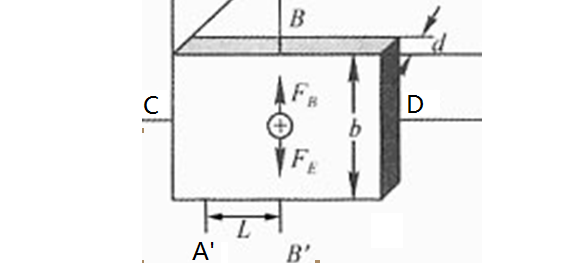
\includegraphics[height=0.27\textheight]{2}

    \hspace{5.8cm}{图3:霍尔效应原理图}

    {
        电导率$\sigma$与载流子浓度n及迁移率$\mu$之间有如下关系;
        \begin{equation}
            \sigma=ne\mu\label{eq:equation2}
        \end{equation}
    }

    \subsection{实验器材}

    {
        两个恒流源, 电磁铁(2400Gs/A), 霍尔器件,
        换向开关和接线柱, 数字万用表, 小磁针.}\label{subsec:3}

    \subsection{实验步骤}\label{subsec:6}

    \noindent{(1)}{
        用六脚霍尔片接好线路,霍尔片的尺寸为:d=0.5mm,b=4.0mm,L=3.0mm。
    }

    \noindent{(2)}{
        保持$I_M$ = $\pm$0.45A不变, $I_S$取$\pm$1.00, 1.50, $\cdots$, 4.50mA,
        测绘$V_H-I_S$曲线,计算$R_H$。
    }

    \noindent{(3)}{
        保持$I_S = \pm4.50mA$不变, $I_M$取$\pm$0.100, 0.150, $\cdots$, 0.45A,
        测绘$V_H-I_M$曲线,计算$R_H$。
    }

    \noindent{(4)}{
        在零磁场下,取$I_S = 1.00mA$,测沿电流方向电势差$V_{xx}$。
    }

    \noindent{(5)}{
        确定样品导电类型, 并求$R_H$, n, $\sigma$, $\mu$。
    }

    \noindent{(6)}{
        用四脚锑化铟片,取 $I_S = 1.00mA$,
        $I_M$在0-0.800A之间,测绘锑化铟片$V_H-I_M$曲线。
    }


    \section{实验结果与讨论}\label{sec:2}

    \subsection{保持励磁电流不变测量霍尔系数}\label{subsec:8}

    \subsubsection{原始数据}
    \begin{table}[h!]
        \centering
        \caption{保持励磁电流不变测量霍尔系数($V_H-I_S$)}
        \begin{tabular}{|c|c|c|c|c|c|c|c|}
            \hline
            \multicolumn{4}{|c|}{$I_M^{ideal}=0.45A\quad I_M^{real}=0.4497A$} & \multicolumn{4}{|c|}{$I_M^{ideal}=-0.45A \quad I_M^{real}=-0.4497A$} \\
            \hline
            $I_S(mA)$ & $V_1(mV)$ & $I_S(mA)$ & $V_1(mV)$ & $I_S(mA)$ & $V_1(mV)$ & $I_S(mA)$ & $V_1(mV)$ \\
            \hline
            1.00      & 1.33      & -0.99     & -1.32     & 1.00      & -1.35     & -0.99     & 1.35      \\
            \hline
            1.48      & 1.95      & -1.48     & -1.94     & 1.48      & -1.97     & -1.48     & 1.98      \\
            \hline
            1.98      & 2.59      & -1.98     & -2.58     & 1.98      & -2.63     & -1.98     & 2.63      \\
            \hline
            2.48      & 3.23      & -2.48     & -3.22     & 2.48      & -3.28     & -2.48     & 3.29      \\
            \hline
            2.98      & 3.88      & -2.98     & -3.87     & 2.98      & -3.93     & -2.98     & 3.94      \\
            \hline
            3.47      & 4.50      & -3.47     & -4.50     & 3.47      & -4.57     & -3.47     & 4.58      \\
            \hline
            3.97      & 5.14      & -3.97     & -5.13     & 3.97      & -5.22     & -3.97     & 5.14      \\
            \hline
            4.47      & 5.78      & -4.47     & -5.77     & 4.47      & -5.88     & -4.47     & 5.89      \\
            \hline
        \end{tabular}\label{tab:table}
    \end{table}

    \subsubsection{数据处理}

    {根据$V_H = \frac{V_1+V_2+V_3+V_4}{4}$计算得到:}

    \begin{tabular}{|c|c|}
        \hline
        $I_S(mA)$ & $V_H(mV)$ \\
        \hline
        1.00      & 1.3375    \\
        \hline
        1.48      & 1.9600    \\
        \hline
        1.98      & 2.6075    \\
        \hline
        2.48      & 3.2550    \\
        \hline
        2.98      & 3.9050    \\
        \hline
        3.47      & 4.5375    \\
        \hline
        3.97      & 5.1575    \\
        \hline
        4.47      & 5.8300    \\
        \hline
    \end{tabular}

    {{使用Origin作图得到$V_H-I_S$图像如下:}}

    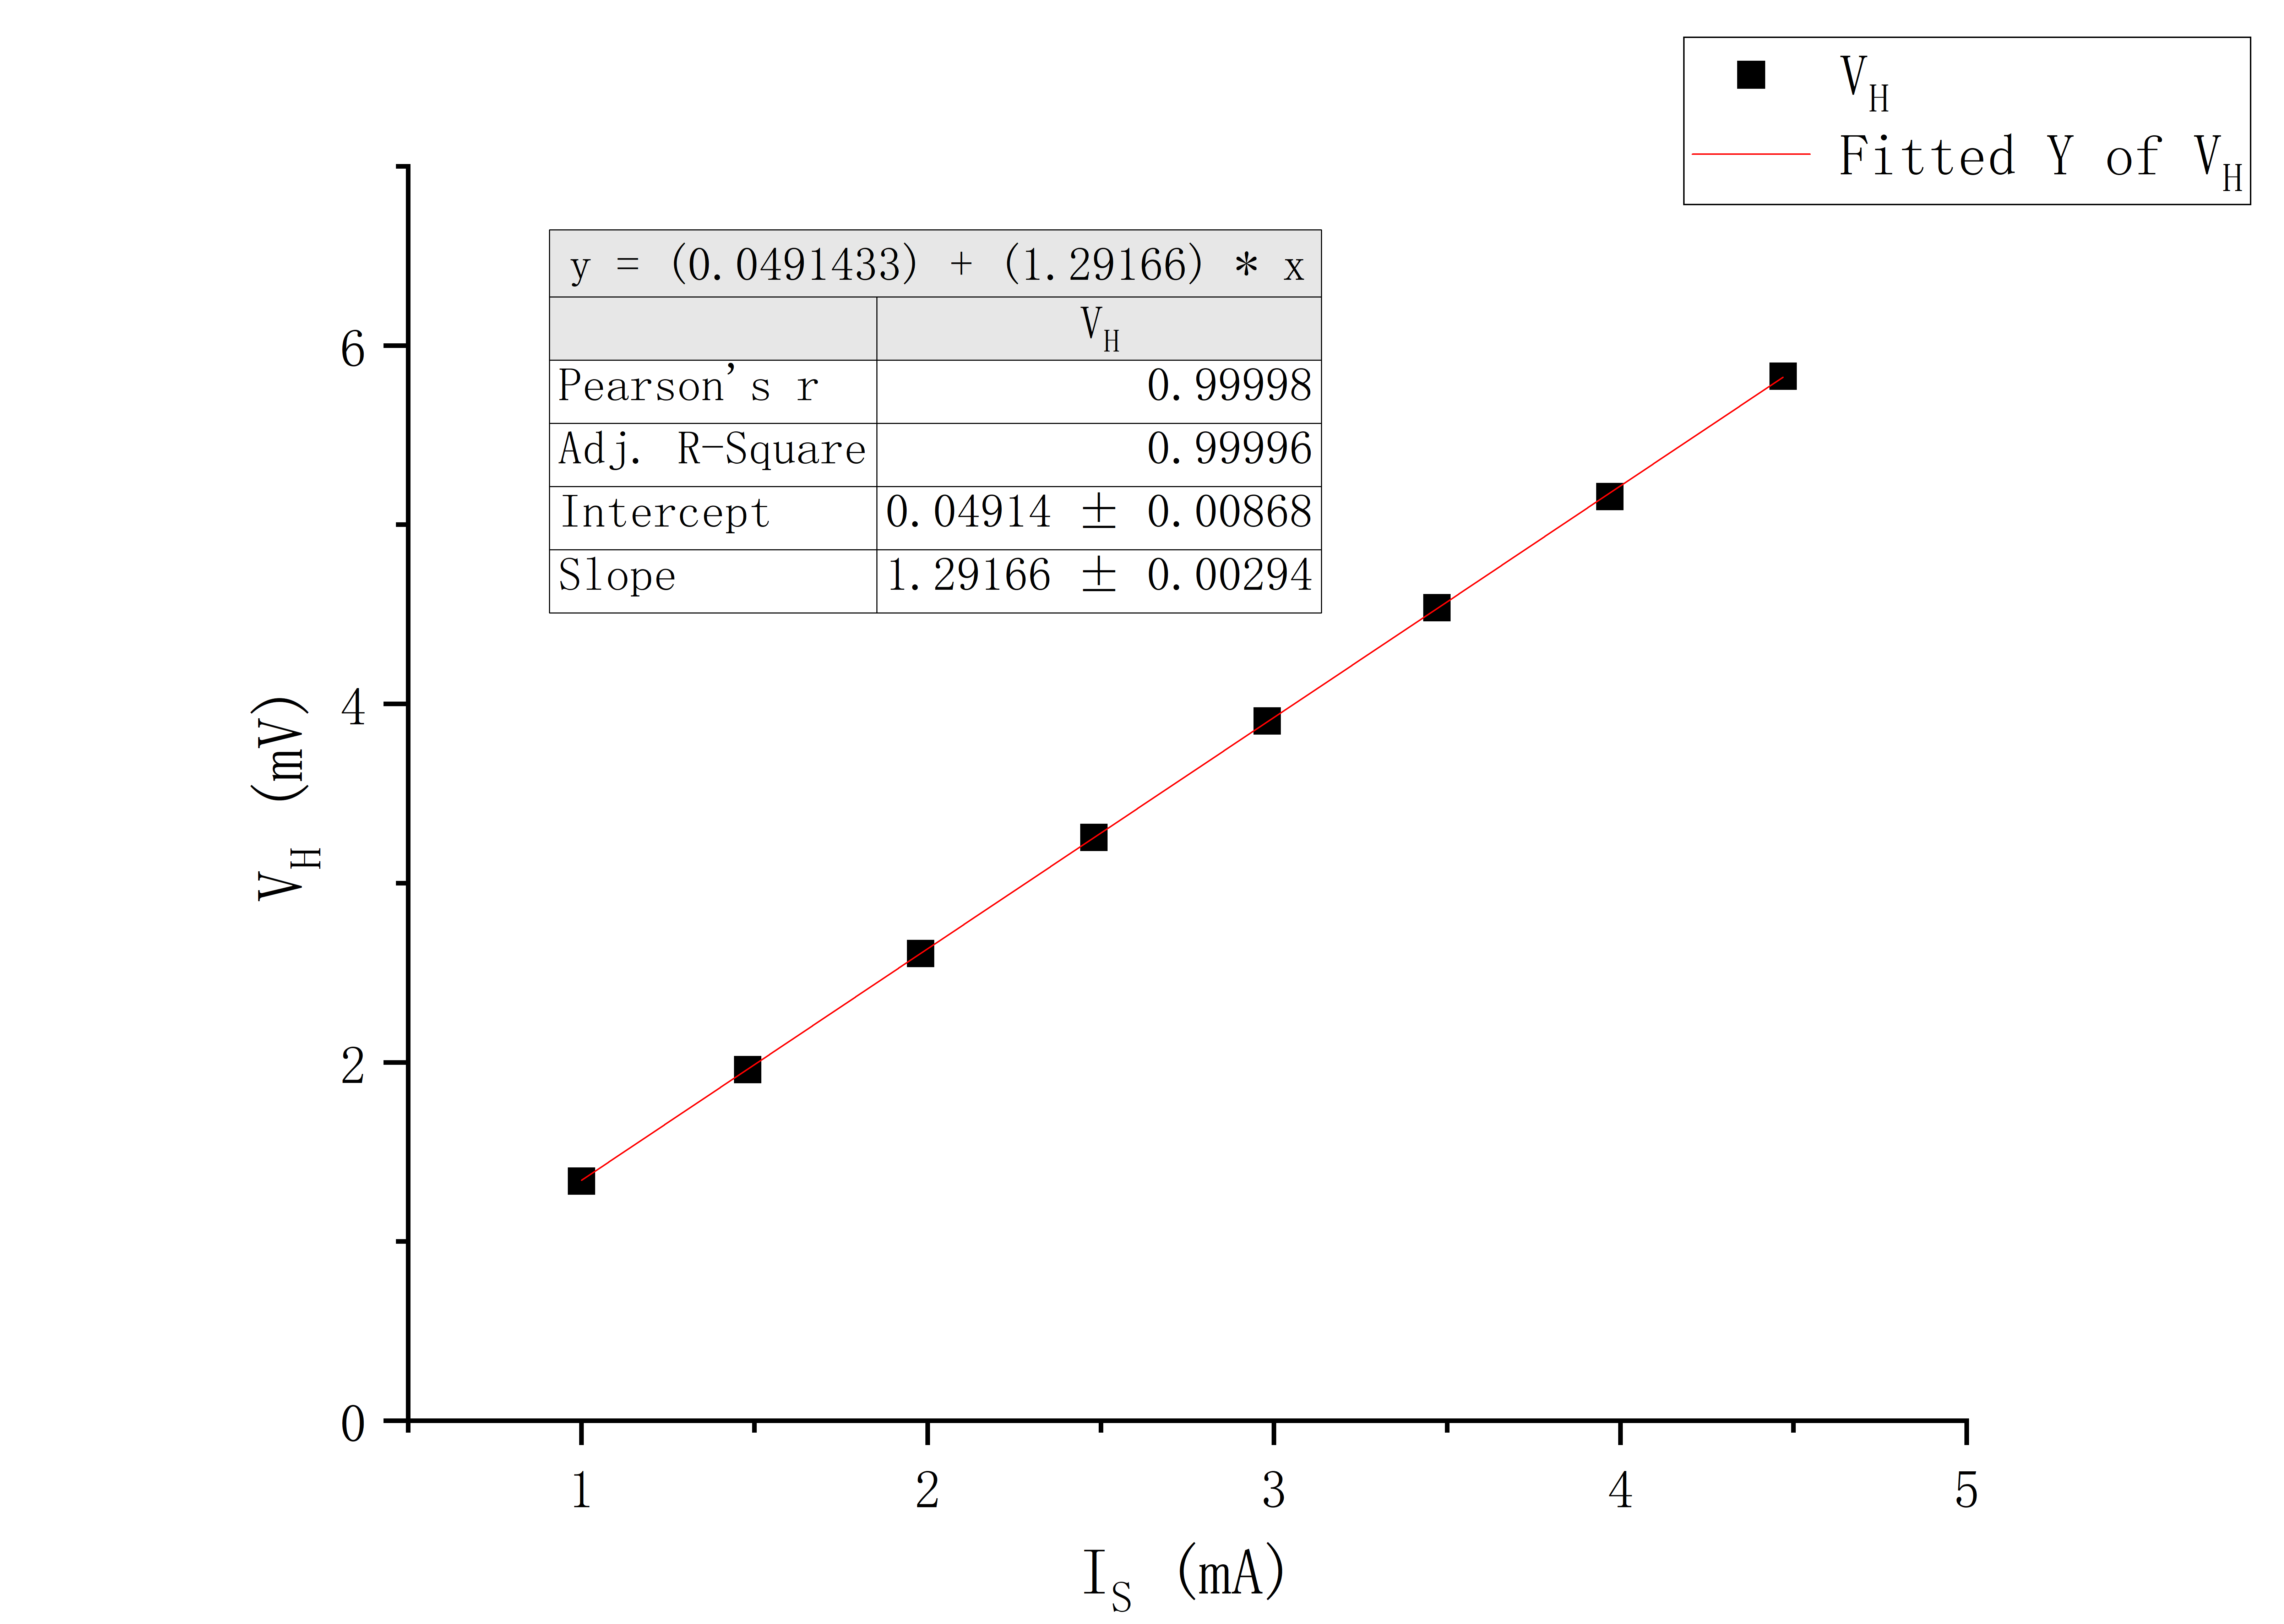
\includegraphics[height=0.4\textheight]{4}

    \hspace{6cm}{图4:$V_H-I_S$}

    {斜率k=1.29V/A,线性拟合$R^2= 0.99998$}
    \begin{flalign}
        \qquad R_H&=\frac{d}{B}\frac{V_H}{I_S}\nonumber&\\
        &=\frac{5\times10^{-4}\times1.29V/A}{2400Gs/A\times0.4497A\times10^{-4}T/Gs}\nonumber\\
        &=5.98\times10^{-3}m^3/C\nonumber
    \end{flalign}

    \subsection{保持样品电流不变测量霍尔系数}\label{subsec:2}

    \subsubsection{原始数据}

    \begin{table}[h!]
        \centering
        \caption{保持样品电流不变测量霍尔系数($V_H-I_M$)}
        \begin{tabular}{|c|c|c|c|c|c|c|c|}
            \hline
            \multicolumn{4}{|c|}{$I_S^{ideal}=4.5mA\quad I_S^{real}=4.47mA$} & \multicolumn{4}{|c|}{$I_S^{ideal}=-4.5mA\quad I_S^{real}=-4.47mA$} \\
            \hline
            $I_M(A)$ & $V_1(mV)$ & $I_M(A)$ & $V_1(mV)$ & $I_M(A)$ & $V_1(mV)$ & $I_M(A)$ & $V_1(mV)$ \\
            \hline
            0.100    & 1.34      & -0.100   & -1.34     & 0.100    & -1.24     & -0.100   & 1.24      \\
            \hline
            0.150    & 1.88      & -0.150   & -1.87     & 0.150    & -1.96     & -0.150   & 1.97      \\
            \hline
            0.200    & 2.50      & -0.200   & -2.50     & 0.200    & -2.60     & -0.200   & 2.61      \\
            \hline
            0.250    & 3.14      & -0.250   & -3.14     & 0.250    & -3.23     & -0.250   & 3.23      \\
            \hline
            0.300    & 3.77      & -0.300   & -3.76     & 0.300    & -3.88     & -0.300   & 3.88      \\
            \hline
            0.350    & 4.43      & -0.350   & -4.42     & 0.350    & -4.50     & -0.350   & 4.51      \\
            \hline
            0.400    & 5.05      & -0.400   & -5.04     & 0.400    & -5.17     & -0.400   & 5.18      \\
            \hline
            0.450    & 5.77      & -0.450   & -5.77     & 0.450    & -5.80     & -0.450   & 5.80      \\
            \hline
        \end{tabular}\label{tab:table1}
    \end{table}
    \subsubsection{数据处理}

    {根据$V_H = \frac{V_1+V_2+V_3+V_4}{4}$计算得到:}

    \begin{tabular}{|c|c|}
        \hline
        $I_M(A)$ & $V_H(mV)$ \\
        \hline
        0.100    & 1.2900    \\
        \hline
        0.150    & 1.9200    \\
        \hline
        0.200    & 2.5525    \\
        \hline
        0.250    & 3.185     \\
        \hline
        0.300    & 3.8825    \\
        \hline
        0.350    & 4.4650    \\
        \hline
        0.400    & 5.0988    \\
        \hline
        0.450    & 5.7850    \\
        \hline
    \end{tabular}

    \vspace{1cm}

    {使用Origin作图得到$V_H-I_M$图像如下:}

    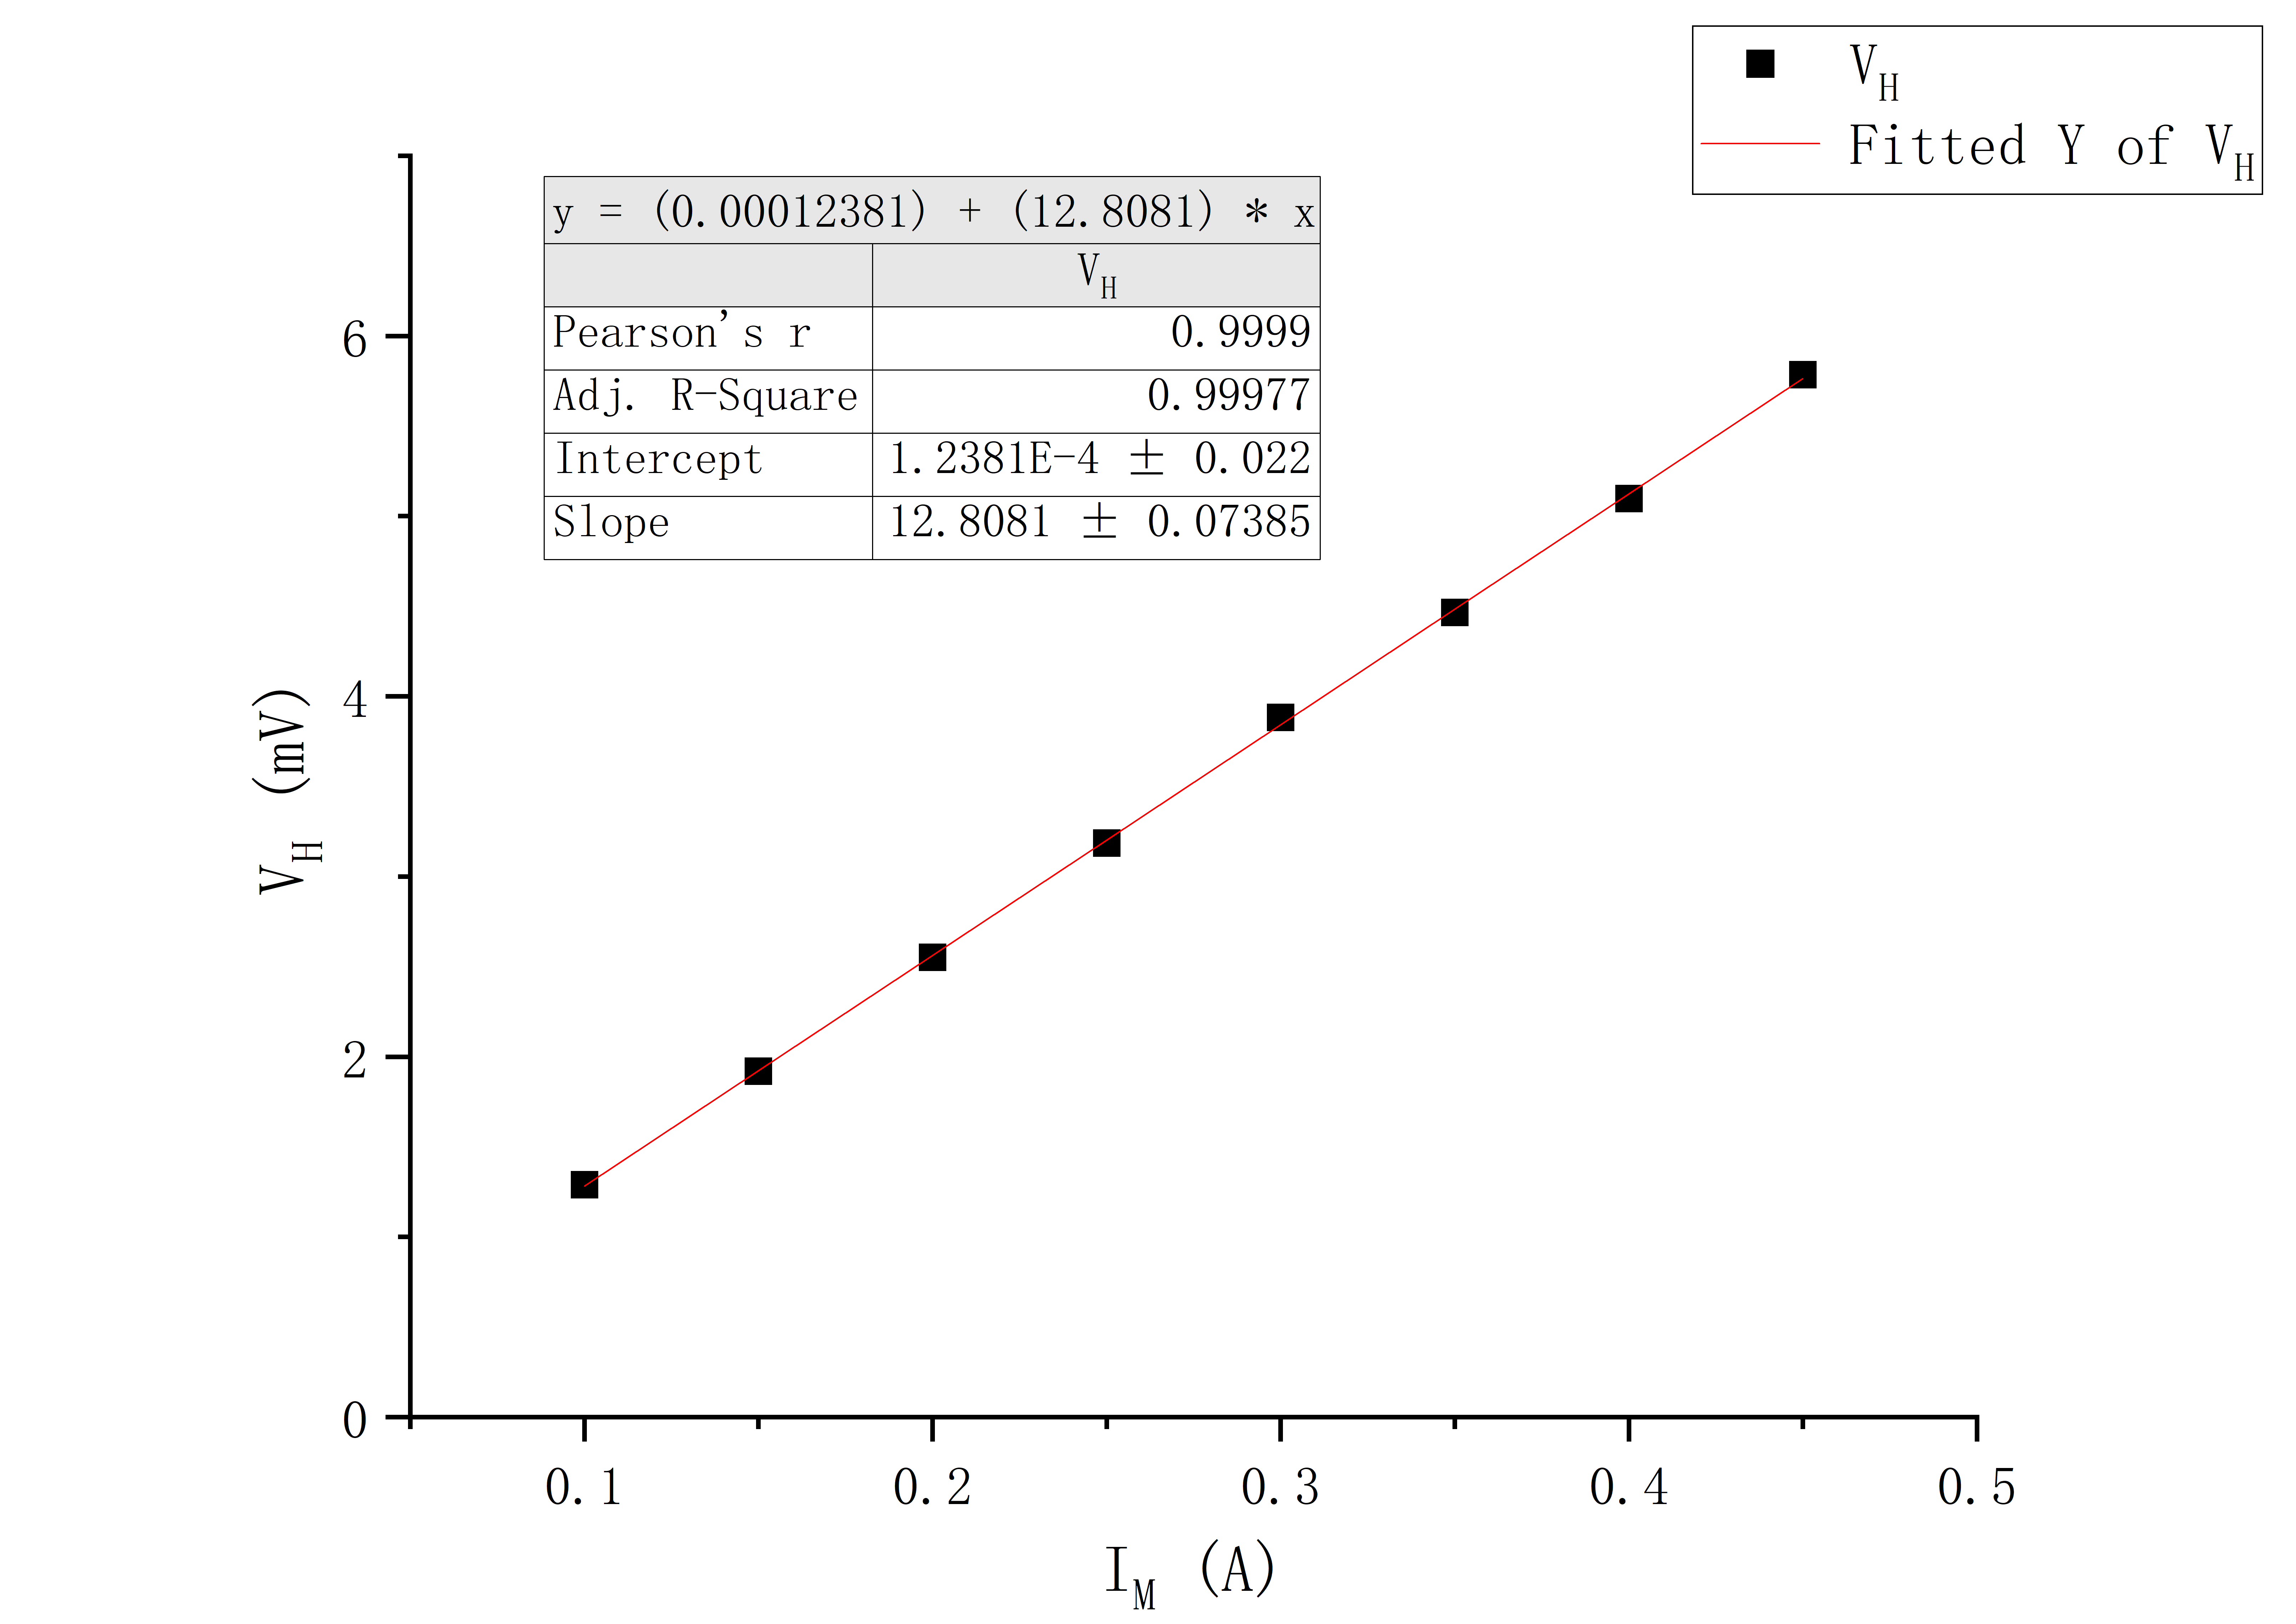
\includegraphics[height=0.4\textheight]{3}

    \hspace{6cm}{图5:$V_H-I_M$}

    {斜率k=12.81mV/A,线性拟合$R^2= 0.99977$}
    \begin{flalign}
        \qquad R_H&=\frac{d}{B}\frac{V_H}{I_S}\nonumber&\\
        &=\frac{5\times10^{-7}m\times12.81V/A}{2400Gs/A\times0.00447A\times10^{-4}T/Gs}\nonumber\\
        &=5.68\times10^{-3}m^3/C\nonumber
    \end{flalign}

    \vspace{2cm}

    \subsection{零磁场下测量横向电势差}
    {
        零磁场下, $I_S=0.99mA$,
    }

    {
        测得$V_{B'A'1}=-59.29mV;V_{B'A'2}=59.14mV$, 则横向电势差为:
    }\label{subsec:1}
    \begin{flalign}
        \qquad V_{xx}&=\frac{|V_{B'A'1}|+|V_{B'A'2}|}{2}=59.215mV\nonumber&
    \end{flalign}

    {{即$V_{B'A'}=59.215mV$}}

    \subsection{判断六脚霍尔元件的导电类型}
    {根据实验1中测量的数据, 在不通电流时,
        小磁针N极指向操作者, 当$I_M>0,I_S>0$,
        此时小磁针N极再次指向实验操作者, 此时电流与磁场关系如下图所示:}\label{subsec:}

    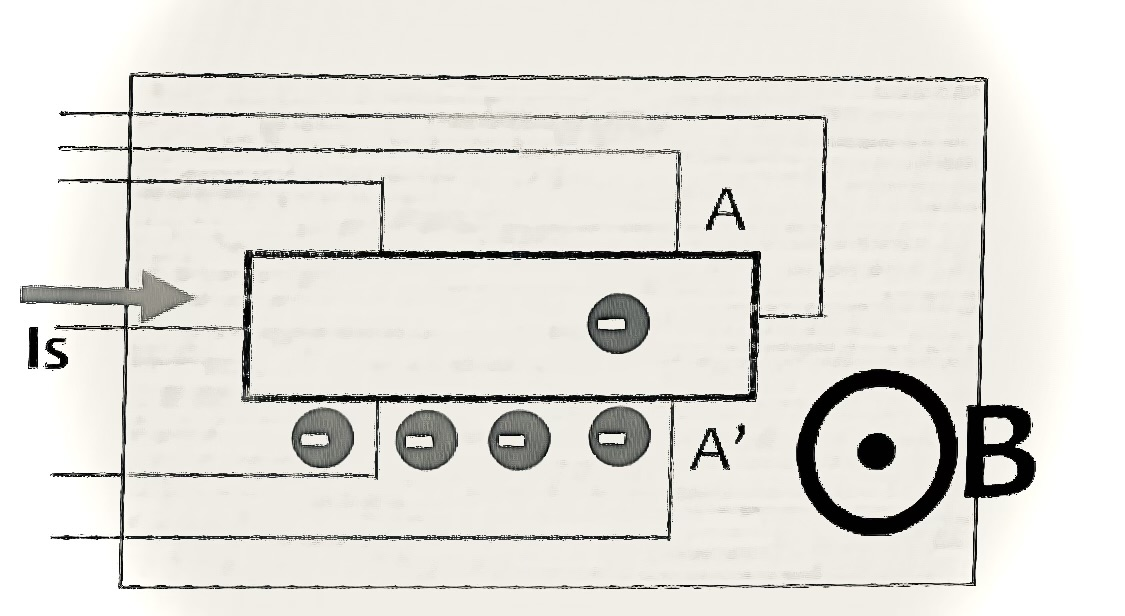
\includegraphics[height=0.2\textheight]{6}

    \hspace{4cm}{\small 图6}

    {又因为此时$V_H=V_1>0$, 可判定该霍尔元件导电类型为n型。}

    {可计算n, $\sigma$, $\mu$如下:}
    \begin{flalign}
        \qquad n&=\frac{1}{R_H q}\nonumber&\\
        &=\frac{1}{5.98\time10^{-3}\times1.6\times10^{-19}}\nonumber\\
        &=1.04\times10^{21}\nonumber\\
        \sigma&=\frac{1}{\rho}\nonumber\\
        &=\frac{L}{bd}\frac{I_S}{V_{xx}}\nonumber\\
        &=\frac{3\times0.99}{4\times0.5\times59.215\times10^{-3}}\nonumber\\
        &=25.078S/m\nonumber\\
        \mu&=\frac{\sigma}{nq}\nonumber\\
        &={25.078}{1.04\times10^{21}\times1.6\times10^{-19}}\nonumber\\
        &=0.151m^2/V\cdot s\nonumber
    \end{flalign}

    \subsection{使用锑化铟片, 保持样品电流$I_S= 1mA$ 不变, 绘制$V_H - I_M$图像}\label{subsec:-$i_s=-1ma$--$v_h---i_m$}

    \begin{tabular}{|c|c|c|c|}
        \hline
        $I_M(A)$ & $V_H(mV)$ & $I_M(A)$ & $V_H(mV)$ \\
        \hline
        0        & 2.40      & 0.44     & 213.12    \\
        \hline
        0.04     & 26.43     & 0.48     & 221.07    \\
        \hline
        0.08     & 50.13     & 0.52     & 228.95    \\
        \hline
        0.12     & 73.15     & 0.56     & 236.56    \\
        \hline
        0.16     & 95.65     & 0.60     & 245.73    \\
        \hline
        0.20     & 117.48    & 0.64     & 256.63    \\
        \hline
        0.24     & 138.61    & 0.68     & 263.56    \\
        \hline
        0.28     & 158.69    & 0.72     & 270.31    \\
        \hline
        0.32     & 177.25    & 0.76     & 277.45    \\
        \hline
        0.36     & 193.02    & 0.80     & 284.87    \\
        \hline
        0.40 & 204.11 & \multicolumn{2}{c|}{ } \\
        \hline
    \end{tabular}

    \vspace{1cm}

    {使用Origin作图得到$V_H-I_M$图像如下:}

    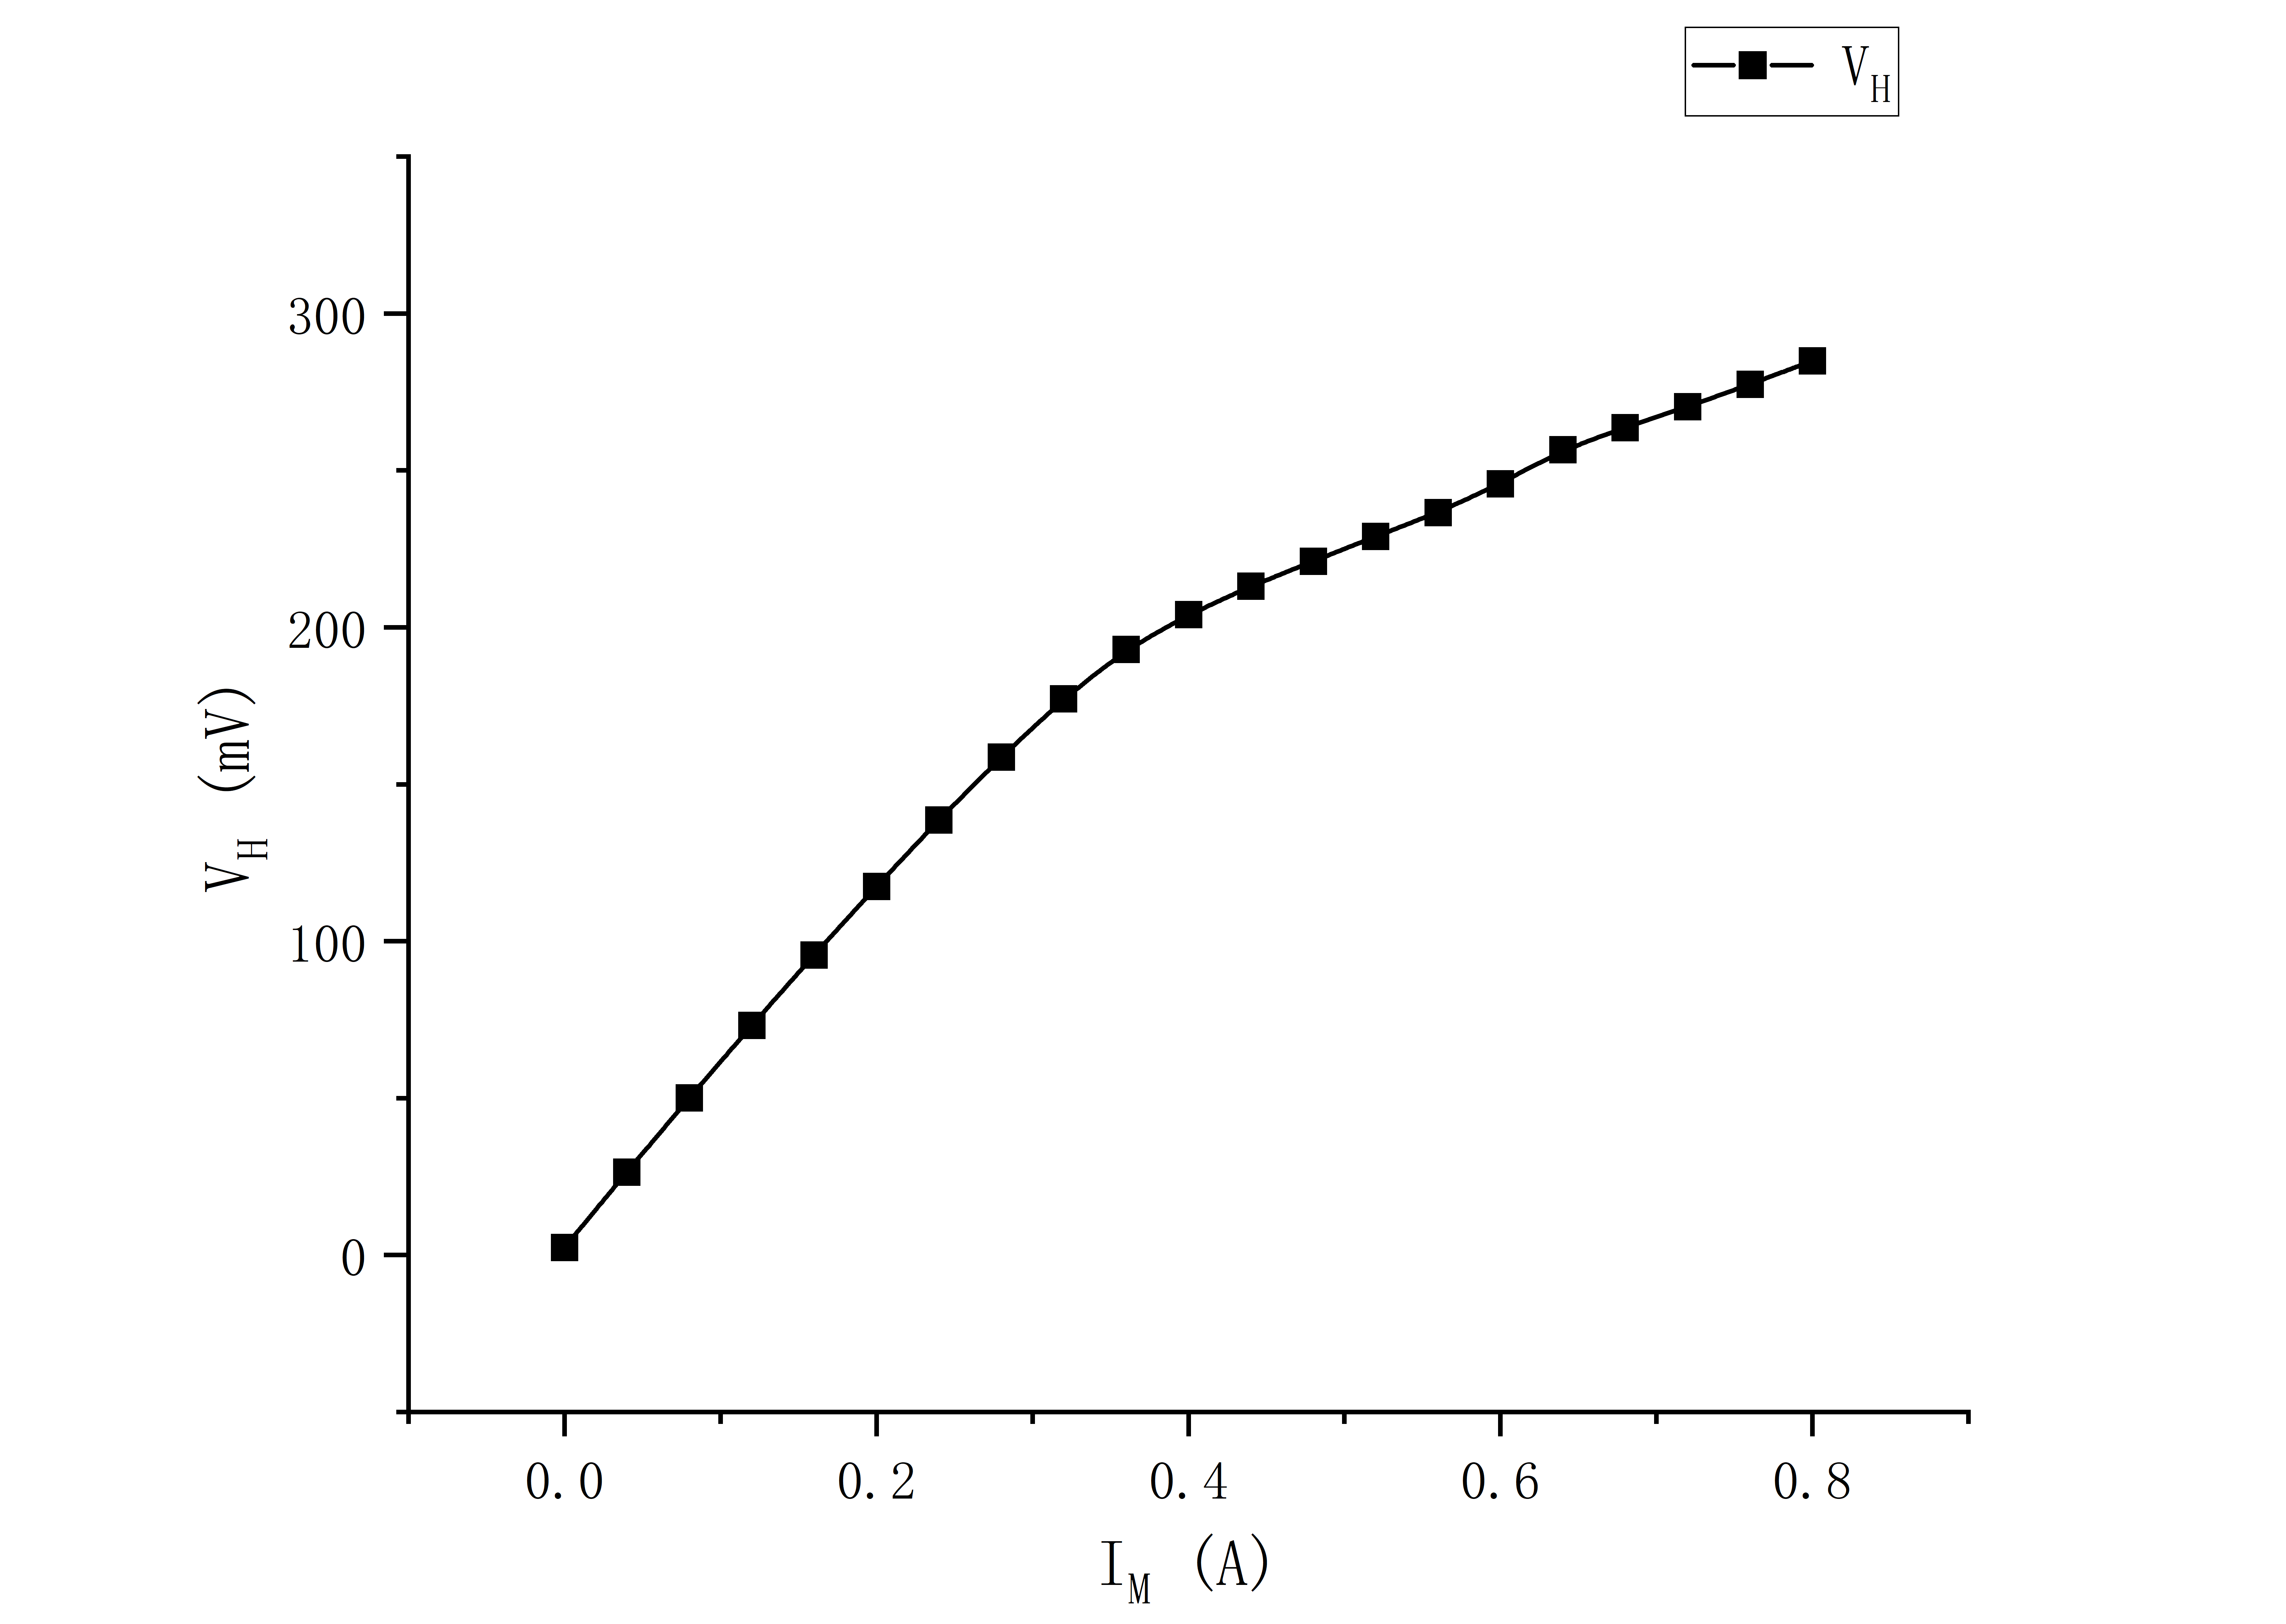
\includegraphics[height=0.4\textheight]{5}

    \hspace{6cm}{图7:$V_H-I_M$}

    \section{实验总结}

    {
        本实验对霍尔效应进行研究并利用霍尔效应进行各种分析和测量工作,
        测量了霍尔片的霍尔系数,
        掌握了载流子类型的判断方法,
        计算了横向电导率、载流子浓度和载流子迁移率,
        了解了各种类型的霍尔效应并认识了其副效应,
        实践了使用对称测量法来消除副效应的方法,
        绘制了锑化铟片的$V_H - I_M$曲线,
        加强了对霍尔效应的认识,
        对后续电磁学理论的学习有重要帮助。
    }\label{sec:1}

    \section{参考文献}

    {[1]中国科学技术大学物理实验教学中心. 霍尔定律(实验讲义).}

    {[2]胡友秋、程福臻.电磁学与电动力学(下册)第二版.
    科学出版社,北京, 2014.}

    {[3]谢行恕,康世秀,霍剑青.大学物理实验,第二册,第二版.
    高等教育出版社,北京, 2005.}\label{sec:}

\end{document}

